\chapter{Specifikacija programske potpore}
		
	\section{Funkcionalni zahtjevi}
			
			\textbf{\textit{dio 1. revizije}}\\
			
			\textit{Navesti \textbf{dionike} koji imaju \textbf{interes u ovom sustavu} ili  \textbf{su nositelji odgovornosti}. To su prije svega korisnici, ali i administratori sustava, naručitelji, razvojni tim.}\\
				
			\textit{Navesti \textbf{aktore} koji izravno \textbf{koriste} ili \textbf{komuniciraju sa sustavom}. Oni mogu imati inicijatorsku ulogu, tj. započinju određene procese u sustavu ili samo sudioničku ulogu, tj. obavljaju određeni posao. Za svakog aktora navesti funkcionalne zahtjeve koji se na njega odnose.}\\
			
			
			\noindent \textbf{Dionici:}
			
			\begin{packed_enum}
				
				\item Zdravstvena ustanova
				\item Prijevoznik			
				\item Vlasnik smještaja
				\item Administrator
				\begin{packed_enum}
					\item Smještajni administrator
					\item Administrator prijevoznih usluga
					\item Korisnički administrator
				\end{packed_enum}
				\item Korisnik
				\item Razvojni tim
				
			\end{packed_enum}
			\pagebreak
			
			\noindent \textbf{Aktori i njihovi funkcionalni zahtjevi:}
			
			
			\begin{packed_enum}
				
				\item \underbar{Administrator (inicijator)  se može:}
				
				\begin{packed_enum}
					\item prijaviti u sustav nakon čega dobija dobija ovlasti ovisno u koje sve vrste administratora spada (smještajni administrator, administrator \mbox{prijevoznih} usluga, korisnički administrator)
					
				\end{packed_enum}		
				
				\item  \underbar{Smještajni administrator (inicijator) može:}
				
				\begin{packed_enum}
					
					\item definirati nove smještajne kapacitete
					\item mijenjati osnovne podatke smještaja (tip stana, kategorija opremljenosti, adresa, vremenski period dostupnosti)
					\item obrisati smještaj
					\item definirati druge korisnike i dodijeliti im uloge (dodavanje novih admina)		
					
				\end{packed_enum}
				
				
				
				\item  \underbar{Administrator prijevoznih usluga (inicijator) može:}
				
				\begin{packed_enum}
					
					\item unositi podatke o prijevoznicima (osnovni osobni podatci prijevoznika, kontakt podatci prijevoznika, vrsta i kapacitet prijevoznog sredstva, radno vrijeme u kojem su raspoloživi)
					\item obrisati prijevoznika
					\item mijenjati neosnovne podatke o prijevozniku
					
				\end{packed_enum}
				
				\item \underbar{Korisnički administrator (inicijator) može:}
				
				\begin{packed_enum}
					
					\item unositi podatke o korisnicima medicinskih usluga (ime, prezime, kontakt, vrijeme i mjesto dolaska/odlaska, preferencije za veličinu i kvalitetu smještaja)
					
					
				\end{packed_enum}
				
				\pagebreak
				
				
				\item \underbar{Baza podataka (sudionik):}
				
				\begin{packed_enum}
					
					\item pohranjuje sve podatke o administratorima i njihovim ovlastima
					\item  pohranjuje sve podatke o korisnicima, smještaju i prijevoznicima
					\item nakon unosa novog korisnika od korisničkog admina, pridjeljuje se raspoloživa smještajna jedinica i označava se zauzetom u tom periodu
					\item periodički provjerava status unosa medicinskih termina komunikacijom s aplikacijom medicinskih usluga
					\item kada se primi odgovor o zaključanom planu medicinskih usluga s listom termina, pridjeljuju se raspoloživi prijevoznici i označavaju se zauzetim. Zatim se šalju poruke elektronične pošte svakom od prijevoznikom s kontaktnim podatcima korisnika kao i o vremenima i adresama smještaja korisnika, te korisniku usluge poruka sa podatcima o prijevoznicima i smještaju
					
				\end{packed_enum}
				
				\item \underbar{API medicinskih usluga (sudionik):}
				
				\begin{packed_enum}
					
					\item detalji tretmana se preuzimaju iz aplikacije za evidenciju medicinskih usluga
					
				\end{packed_enum}
				
				
				\item \underbar{Google Maps (sudionik):}
				
				\begin{packed_enum}
					
					\item preko podakata o smještaju omogućava grafički prikaz lokacije smještaja
					
				\end{packed_enum}
				
			\end{packed_enum}
			
			\eject 
			
			
				
			\subsection{Obrasci uporabe}
				
				\textbf{\textit{dio 1. revizije}}
				
				\subsubsection{Opis obrazaca uporabe}
					\textit{Funkcionalne zahtjeve razraditi u obliku obrazaca uporabe. Svaki obrazac je potrebno razraditi prema donjem predlošku. Ukoliko u nekom koraku može doći do odstupanja, potrebno je to odstupanje opisati i po mogućnosti ponuditi rješenje kojim bi se tijek obrasca vratio na osnovni tijek.}\\
					

					\noindent \underbar{\textbf{UC1 - Prijava}}
					\begin{packed_item}
	
						\item \textbf{Glavni sudionik: } Administrator
						\item  \textbf{Cilj:} Prijava administratora u sustav
						\item  \textbf{Sudionici:} Administrator i baza podataka
						\item  \textbf{Preduvjet:} Nema
						\item  \textbf{Opis osnovnog tijeka:}
						
						\item[] \begin{packed_enum}
	
							\item Otvaranje aplikacije unutar web preglednika
							\item Unos korisničkog imena i lozinke
							\item Podnošenje zahtjeva za prijavu klikom na gumb
							\item Korisnik biva preusmjeren na početnu stranicu
						\end{packed_enum}
						
						\item  \textbf{Opis mogućih odstupanja:}
						
						\item[] \begin{packed_item}
	
							\item[2.a] Uneseni podatci ne odgovaraju traženom formatu
							\item[] \begin{packed_enum}
								
								\item Ispis upozorenja o krivom formatu i onemogućen gumb za prijavu sve dok podatci ne zadovoljavaju traženi format
								
							\end{packed_enum}

							\item[4.a] Korisnički podatci su neispravni ili nisu prepoznati u bazi podataka
							\item[] \begin{packed_enum}
								
								\item Korisnika ne preusmjeravamo na početnu stranicu već mu samo ispisujemo da prijava nije uspjela.
								
							\end{packed_enum}
						\end{packed_item}
					\end{packed_item}
					
					%------------------------------------------------------------------------------
					\noindent \underbar{\textbf{UC2 -Dodavanje novog administratora}}
					\begin{packed_item}
						
						\item \textbf{Glavni sudionik: }Smještajni administrator
						\item  \textbf{Cilj:} Dodati korisničke podatke novog administratora i dodijeliti mu odgovarajuće uloge
						\item  \textbf{Sudionici:} Smještajni administrator i baza podataka
						\item  \textbf{Preduvjet:} UC1: Prijava
						\item  \textbf{Opis osnovnog tijeka:}
						
						\item[] \begin{packed_enum}
							
							\item Administrator odabire opciju za dodavanje novog administratora
							\item Unosi korisničke podatke novog administratora
							\item Označuje uloge dodijeljene novom administratoru
							\item Podnosi zahtjev za unosom novog administratora u bazu podataka
							\item Sva polja se postavljaju na početne vrijednosti
							
						\end{packed_enum}
						
						\item  \textbf{Opis mogućih odstupanja:}
						
						\item[] \begin{packed_item}
							
							\item[2.a] Uneseni podatci ne odgovaraju traženom formatu
							\item[] \begin{packed_enum}
								
								\item Ispis upozorenja o krivom formatu i onemogućen gumb za dodavanje novog administratora sve dok podatci ne zadovoljavaju traženi format
								
							\end{packed_enum}

							\item[3.a] Nije označena ni jedna uloga
							\item[] \begin{packed_enum}
								
								\item Onemogućen gumb za dodavanje novog administratora sve dok nije označena barem jedna uloga novog administratora
								
							\end{packed_enum}
							
							\item[4.a] Sustav vraća grešku prilikom dodavanja novog administratora
							\item[] \begin{packed_enum}
								
								\item Ispisati tekst greške
								\item Čekati na novi pokušaj podnošenja zahtjeva(Korak 4.)
								
							\end{packed_enum}
							
						\end{packed_item}
					\end{packed_item}
					
					%------------------------------------------------------------------------------
					\noindent \underbar{\textbf{UC3 -Unos raspoloživog smještaja}}
					\begin{packed_item}
						
						\item \textbf{Glavni sudionik: }Smještajni administrator
						\item  \textbf{Cilj:} Unos novog smještaja u bazu podataka
						\item  \textbf{Sudionici:} Smještajni administrator i baza podataka
						\item  \textbf{Preduvjet:} UC1: Prijava
						\item  \textbf{Opis osnovnog tijeka:}
						
						\item[] \begin{packed_enum}
							
							\item Administrator odabire opciju za dodavanje novog smještaja
							\item Odabir tipa stana
							\item Odabir kategorije stana 
							\item Unos maksimalnog kapaciteta stana
							\item Unos adrese na kojoj se stan nalazi(UC4)
							\item Unos podataka o zgradi(Broj kata, broj stana, dostupnost lifta, opis)
							\item Odabir tipa vlasništva
							
						\end{packed_enum}
						
						\item  \textbf{Opis mogućih odstupanja:}
						
						\item[] \begin{packed_item}
							
							\item[2.a] Nije odabran ni jedan tip stana
							\item[] \begin{packed_enum}
								
								\item Onemogućeno podnošenje zahtjeva za dodavanjem smještaja u bazu
								\item Ispis upozorenja o odabiru
								
							\end{packed_enum}
							
							\item[3.a] Nije odabran ni jedna kategorija stana
							\item[] \begin{packed_enum}
								
								\item Onemogućeno podnošenje zahtjeva za dodavanjem smještaja u bazu
								\item Ispis upozorenja o odabiru
								
							\end{packed_enum}
							
							\item[4.a] Uneseni podatak nije u odgovarajućem formatu
							\item[] \begin{packed_enum}
								
								\item Onemogućeno podnošenje zahtjeva za dodavanjem smještaja u bazu
								\item Ispis greške o krivom formatu
								
							\end{packed_enum}
							
							\item[7.a] Odabran tip privatnog vlasništva
							\item[] \begin{packed_enum}
								
								\item Unos podataka vezanih za stan u vlasništvu(UC3.1)
								
							\end{packed_enum}
							
							\item[7.b] Odabran tip stana u najmu
							\item[] \begin{packed_enum}
								
								\item Unos podataka vezanih za stan u najmu(UC3.2)
								
							\end{packed_enum}
							
						\end{packed_item}
					\end{packed_item}
					
					%------------------------------------------------------------------------------
					\noindent \underbar{\textbf{UC3.1 -Smještaj u vlasništvu}}
					\begin{packed_item}
						
						\item \textbf{Glavni sudionik: }Smještajni administrator
						\item  \textbf{Cilj:} Unos podataka o smještaju u vlasništvu
						\item  \textbf{Sudionici:} Smještajni administrator i baza podataka
						\item  \textbf{Preduvjet:} UC1: Prijava i UC3: Unos raspoloživog smještaja
						\item  \textbf{Opis osnovnog tijeka:}
						
						\item[] \begin{packed_enum}
							
							\item Podnošenje zahtjeva za dodavanje smještaja u bazu podataka
							\item Preusmjeravanje na početnu stranicu
							
						\end{packed_enum}
						
						\item  \textbf{Opis mogućih odstupanja:}
						
						\item[] \begin{packed_item}
							
							\item[1.a] Dogodila se greška prilikom dodavanja smještaja
							\item[] \begin{packed_enum}
								
								\item Ispis teksta greške administratoru
								\item Povratak na 1. korak
								
							\end{packed_enum}
							
						\end{packed_item}
					\end{packed_item}
					
					%------------------------------------------------------------------------------
					\noindent \underbar{\textbf{UC3.2 -Smještaj u najmu}}
					\begin{packed_item}
						
						\item \textbf{Glavni sudionik: }Smještajni administrator
						\item  \textbf{Cilj:} Unos podataka o smještaju u najmu
						\item  \textbf{Sudionici:} Smještajni administrator i baza podataka
						\item  \textbf{Preduvjet:} UC1: Prijava i UC3: Unos raspoloživog smještaja
						\item  \textbf{Opis osnovnog tijeka:}
						
						\item[] \begin{packed_enum}
							
							\item Unos vremena dostupnosti stana
							\item Podnošenje zahtjeva za dodavanje smještaja u bazu podataka
							\item Preusmjeravanje na početnu stranicu
							
						\end{packed_enum}
						
						\item  \textbf{Opis mogućih odstupanja:}
						
						\item[] \begin{packed_item}
							
							\item[1.a] Nije uneseno vrijeme dostupnosti
							\item[] \begin{packed_enum}
								
								\item Onemogućeno podnošenje zahtjeva za dodavanje smještaja u bazi
								\item Ispis greške o dostupnosti
								
							\end{packed_enum}
							
							\item[2.a] Dogodila se greška prilikom dodavanja smještaja
							\item[] \begin{packed_enum}
								
								\item Ispis teksta greške administratoru
								\item Povratak na 2. korak
								
							\end{packed_enum}
							
						\end{packed_item}
					\end{packed_item}
					
					%------------------------------------------------------------------------------
					\noindent \underbar{\textbf{UC4 -Odabir lokacije}}
					\begin{packed_item}
						
						\item \textbf{Glavni sudionik: }Smještajni administrator
						\item  \textbf{Cilj:} Unos podataka o lokaciji i prikaz lokacije na karti
						\item  \textbf{Sudionici:} Smještajni administrator i \textit{Google Maps}
						\item  \textbf{Preduvjet:} UC1: Prijava
						\item  \textbf{Opis osnovnog tijeka:}
						
						\item[] \begin{packed_enum}
							
							\item Unos podataka o lokaciji(Grad, ulica, kućni broj)
							\item Prikaz unesene lokacije na krati pomoću servisa \textit{Google Maps}
							
						\end{packed_enum}
						
						\item  \textbf{Opis mogućih odstupanja:}
						
						\item[] \begin{packed_item}
							
							\item[1.a] Podatci ne odgovaraju traženom formatu
							\item[] \begin{packed_enum}
								
								\item Ne upućujemo zahtjev na \textit{Google Maps}
								\item Onemogućen odabir lokacije
								\item Ispis greške u podacima
								
							\end{packed_enum}
							
							\item[2.a] Dogodila se greška prilikom prikaza lokacije
							\item[] \begin{packed_enum}
								
								\item Onemogućen odabir lokacije
								\item Ispis greške dobivene od \textit{Google Mapsa}
								
							\end{packed_enum}
							
						\end{packed_item}
					\end{packed_item}
					
					%------------------------------------------------------------------------------
					\noindent \underbar{\textbf{UC5 -Pregled podataka u bazi}}
					\begin{packed_item}
						
						\item \textbf{Glavni sudionik:} Administrator
						\item  \textbf{Cilj:} Pregled svih unesenih podataka u bazi
						\item  \textbf{Sudionici:} Administrator i baza podataka
						\item  \textbf{Preduvjet:} UC1: Prijava
						\item  \textbf{Opis osnovnog tijeka:}
						
						\item[] \begin{packed_enum}
							
							\item Administrator odabire koju grupu podataka hoće vidjeti
							\item Ako administrator odabere filtar ili specificira sortiranje podataka podatci se sortiraju i ponovno prikažu(UC5.1)
							\item Ako administrator odabere brisanje određenog unosa koristi se UC6
							\item Ako administrator odabere uređivanje određenog unosa koristi se UC7
							
						\end{packed_enum}
						
					\end{packed_item}
					
					%------------------------------------------------------------------------------
						\noindent \underbar{\textbf{UC5.1 - Filtriranje i sortiranje podataka za prikaz}}
					\begin{packed_item}
						
						\item \textbf{Glavni sudionik: } Administrator
						\item  \textbf{Cilj:} Pregled sortiranih i filtriranih podataka
						\item  \textbf{Sudionici:} Administrator i baza podataka
						\item  \textbf{Preduvjet:} UC1: Prijava
						\item  \textbf{Opis osnovnog tijeka:}
						
						\item[] \begin{packed_enum}
							
							\item Odabir ponuđenih ograničenja na skup podataka (raspon vrijednosti, podaci specifično grupirani i slično)
							\item Odabir načina sortiranja podataka (uzlazno, silazno)
							\item Prikaz podataka
						\end{packed_enum}
					\end{packed_item}
					
					%------------------------------------------------------------------------------
					
					\noindent \underbar{\textbf{UC6 -Brisanje unosa}}
					\begin{packed_item}
						
						\item \textbf{Glavni sudionik: }Administrator
						\item  \textbf{Cilj:} Brisanje podataka iz baze podataka
						\item  \textbf{Sudionici:} Administrator i baza podataka
						\item  \textbf{Preduvjet:} UC1: Prijava
						\item  \textbf{Opis osnovnog tijeka:}
						
						\item[] \begin{packed_enum}
							
							\item Prikaz odabranog unosa kojeg treba obrisati
							\item Administrator potvrđuje brisanje unosa
							\item Prikaz ažuriranih podataka 
							
						\end{packed_enum}
						
						\item  \textbf{Opis mogućih odstupanja:}
						
						\item[] \begin{packed_item}
							
							\item[2.a] Administrator ne potvrđuje brisanje
							\item[] \begin{packed_enum}
								
								\item Povratak na prikaz podataka bez brisanja
								
							\end{packed_enum}
							
						\end{packed_item}
					\end{packed_item}
					
					%------------------------------------------------------------------------------
					\noindent \underbar{\textbf{UC7 -Promjena podataka}}
					\begin{packed_item}
						
						\item \textbf{Glavni sudionik: }Administrator
						\item  \textbf{Cilj:} Promjena podataka u bazi podataka
						\item  \textbf{Sudionici:} Administrator i baza podataka
						\item  \textbf{Preduvjet:} UC1: Prijava
						\item  \textbf{Opis osnovnog tijeka:}
						
						\item[] \begin{packed_enum}
							
							\item Prikaz promjenjivih podataka odabranog unosa 
							\item Administrator izmjenjuje potrebne podatke
							\item Podnošenje zahtjeva za izmjenom podataka
							
						\end{packed_enum}
						
						\item  \textbf{Opis mogućih odstupanja:}
						
						\item[] \begin{packed_item}
							
							\item[2.a] Novi podatci ne odgovaraju traženom formatu 
							\item[] \begin{packed_enum}
								
								\item Ispis upozorenja o krivom formatu
								\item Onemogućeno podnošenje zahtjeva za promjenom sve dok format nije zadovoljen
								
							\end{packed_enum}
							
							\item[3.a] Administrator odustaje od izmjene podataka
							\item[] \begin{packed_enum}
								
								\item Povratak na prikaz podataka bez slanja zahtjeva za izmjenom podataka
								
							\end{packed_enum}
							
						\end{packed_item}
					\end{packed_item}
					
					%------------------------------------------------------------------------------
					\noindent \underbar{\textbf{UC8 -Unos podataka o prijevoznicima}}
					\begin{packed_item}
						
						\item \textbf{Glavni sudionik: }Prijevozni administrator
						\item  \textbf{Cilj:} Stvoriti novi zapis u bazi podataka s podacima o prijevozniku
						\item  \textbf{Sudionici:} Prijevozni administrator i baza podataka
						\item  \textbf{Preduvjet:} UC1: Prijava
						\item  \textbf{Opis osnovnog tijeka:}
						
						\item[] \begin{packed_enum}
							
							\item Administrator odabire opciju za dodavanje novog prijevoznika
							\item Unos osobnih podataka, kontaktnih podataka i podataka o vozilu
							\item Odabir radnog vremena i radnih dana u tjednu
							\item Podnošenje zahtjeva za upisom prijevoznika u bazu podataka
							
						\end{packed_enum}
						
						\item  \textbf{Opis mogućih odstupanja:}
						
						\item[] \begin{packed_item}
							
							\item[2.a] Podatci ne odgovaraju traženom formatu 
							\item[] \begin{packed_enum}
								
								\item Ispis upozorenja o krivom formatu
								\item Onemogućeno podnošenje zahtjeva za upisom podataka
								
							\end{packed_enum}
							
							\item[3.a] Nije ispravno odabrano radno vrijeme
							\item[] \begin{packed_enum}
								
								\item Ispis upozorenja o krivom radnom vremenu
								\item Onemogućeno podnošenje zahtjeva za upisom podataka
								
							\end{packed_enum}
							
							\item[4.a] Dogodila se greška prilikom upisa podataka u bazu
							\item[] \begin{packed_enum}
								
								\item Ispis teksta greške
								
							\end{packed_enum}
							
						\end{packed_item}
					\end{packed_item}
					
					%------------------------------------------------------------------------------
					\noindent \underbar{\textbf{UC9 -Unos podataka o korisnicima}}
					\begin{packed_item}
						
						\item \textbf{Glavni sudionik: }Korisnički administrator
						\item  \textbf{Cilj:} Stvoriti novi zapis u bazi podataka s podacima o korisniku
						\item  \textbf{Sudionici:} Korisnički administrator i baza podataka
						\item  \textbf{Preduvjet:} UC1: Prijava
						\item  \textbf{Opis osnovnog tijeka:}
						
						\item[] \begin{packed_enum}
							
							\item Administrator odabire opciju za dodavanje novog korisnika
							\item Unos osobnih i kontaktnih podataka
							\item Odabir lokacije dolaska korisnika(UC4)
							\item Odabir vremena dolaska korisnika
							\item Odabir lokacije odlaska korisnika(UC4)
							\item Odabir vremena odlaska korisnika
							\item Odabir preferencija korisnika
							\item Podnošenje zahtjeva za upisom korisnika u bazu podataka
							
						\end{packed_enum}
						
						\item  \textbf{Opis mogućih odstupanja:}
						
						\item[] \begin{packed_item}
							
							\item[2.a] Podatci ne odgovaraju traženom formatu 
							\item[] \begin{packed_enum}
								
								\item Ispis upozorenja o krivom formatu
								\item Onemogućeno podnošenje zahtjeva za upisom podataka
								
							\end{packed_enum}
							
							\item[3.a i 5.a] Nije odabrana lokacija
							\item[] \begin{packed_enum}
								
								\item Onemogućeno podnošenje zahtjeva za upisom podataka
								
							\end{packed_enum}
							
							\item[4.a i 6.a] Nije ispravno odabrano vrijeme dolaska
							\item[] \begin{packed_enum}
								
								\item Ispis upozorenja o krivom unosu vremenu
								\item Onemogućeno podnošenje zahtjeva za upisom podataka
								
							\end{packed_enum}
							
							\item[8.a] Dogodila se pogreška prilikom upisa podataka
							\item[] \begin{packed_enum}
								
								\item Ispis teksta greške
								
							\end{packed_enum}
							
						\end{packed_item}
					\end{packed_item}
					
					%------------------------------------------------------------------------------
					\noindent \underbar{\textbf{UC10 -Usklađivanje podataka}}
					\begin{packed_item}
						
						\item \textbf{Glavni sudionik:} Baza podataka
						\item  \textbf{Cilj:} Uskladiti podatke iz baze podataka s podacima u bazi podataka pružatelja medicinske usluge
						\item  \textbf{Sudionici:} Baza podataka i API medicinske usluge
						\item  \textbf{Preduvjet:} -
						\item  \textbf{Pokretač:} Prošlo je određeno vrijeme od zadnjeg usklađivanja
						\item  \textbf{Opis osnovnog tijeka:}
						
						\item[] \begin{packed_enum}
							
							\item Baza podataka šalje upit API-ju s podacima korisnika za koje nema zabilježen ID
							\item API odgovara s traženim popisom
							\item Baza usklađuje ID-eve iz popisa
							\item Baza podataka šalje upit tražeći popis zaključanih medicinskih termina zabilježenih nakon određenog datuma(Datum zadnjeg usklađivanja podataka)
							\item API odgovara s traženim popisom
							\item Baza podataka obrađuje sve zaključane termine(UC11)
							
						\end{packed_enum}
						
						\item  \textbf{Opis mogućih odstupanja:}
						
						\item[] \begin{packed_item}
							
							\item[1.a] Nema korisnika s nezabilježenim ID-em u bazi podataka
							\item[] \begin{packed_enum}
								
								\item Ne šalje se upit
								\item Prelazimo na korak 4.
								
							\end{packed_enum}
							
							\item[2.a i 5.a] Nismo dobili odgovor 
							\item[] \begin{packed_enum}
								
								\item Nakon 10 sekundi pokušamo ponovno korak 1./4.
								\item U slučaju 3 ili više neuspjeha, šaljemo obavijest smještajnom administratoru(UC10.1)
								\item Prekidamo proces usklađivanja podataka
								
							\end{packed_enum}
							
						\end{packed_item}
					\end{packed_item}
					
					%------------------------------------------------------------------------------
					\noindent \underbar{\textbf{UC10.1 - Slanje obavijesti smještajnom administratoru}}
					\begin{packed_item}
						
						\item \textbf{Glavni sudionik: } Baza podataka
						\item  \textbf{Cilj:} Obavijestiti smještajnog administratora o nemogučnosti usklađivanja s API-em medicinskih usluga
						\item  \textbf{Sudionici:} Baza podataka, smještajni administrator i API medicinskih usluga
						\item  \textbf{Preduvjet:} UC1: Prijava
						\item \textbf{Pokretač: } API ne odgovara na upit 3 ili više puta kod usklađivanja podataka (UC10)
						\item  \textbf{Opis osnovnog tijeka:}
						
						\item[] \begin{packed_enum}
							
							\item Slanje obavijesti smještajnom administratoru na mail s uključenim vremenom i sadržajem upita API-u medicinskih usluga
						\end{packed_enum}
					\end{packed_item}
					
					%------------------------------------------------------------------------------
					\noindent \underbar{\textbf{UC11 -Zaključan plan usluge}}
					\begin{packed_item}
						
						\item \textbf{Glavni sudionik:} Baza podataka
						\item  \textbf{Cilj:} Slanje poruke u obliku emaila korisniku i prijevozniku sa svim potrebnim podacima
						\item  \textbf{Sudionici:} Baza podataka, korisnik i prijevoznik
						\item  \textbf{Preduvjet:} -
						\item  \textbf{Pokretač:} Dobiven zapis o zaključanom terminu tretmana tokom UC10: Usklađivanje podataka
						\item  \textbf{Opis osnovnog tijeka:}
						
						\item[] \begin{packed_enum}
							
							\item Odabir prijevoznika dostupnog u terminu dolaska korisnika \newline(prijevoznik1)
							\item Odabir prijevoznika dostupnog u terminu tretmana $\pm$2h \newline(prijevoznik2)
							\item Odabir prijevoznika dostupnog u terminu odlaska korisnika \newline(prijevoznik3)
							\item Slanje poruke svakom od prijevoznika s potrebnim podacima
							\item Slanje poruke korisniku s podacima ukupnog plana njihovog puta i kontaktnim podacima prijevoznika
							
						\end{packed_enum}
						
						\item  \textbf{Opis mogućih odstupanja:}
						
						\item[] \begin{packed_item}
							
							\item[1.a, 2.a i 3.a] Ne postoji prijevoznik dostupan u tom terminu
							\item[] \begin{packed_enum}
								
								\item Šaljemo obavijest prijevoznom administratoru o nemogućnosti uparivanja prijevoznika s korisnikom
								\item Označavamo taj termin nedovršenim
								\item Čekamo prijevoznog administratora da poduzme akciju(UC11.1)
								
							\end{packed_enum}
							
							\item[4.a] Nisu sva tri prijevoznika različita
							\item[] \begin{packed_enum}
								
								\item Ne šaljemo prijevozniku više od jedne poruke već sve podatke vezane za tog prijevoznika grupiramo u jednu poruku
								
							\end{packed_enum}
							
						\end{packed_item}
					\end{packed_item}
					
					%------------------------------------------------------------------------------
					
					\noindent \underbar{\textbf{UC11.1 - Slanje obavijesti prijevoznom administratoru}}
					\begin{packed_item}
						
						\item \textbf{Glavni sudionik: } Baza podataka
						\item  \textbf{Cilj:} Obavijestiti prijevoznog administratora o nepostojanju prijevoznika s odabranim terminom
						\item  \textbf{Sudionici:} Baza podataka, prijevozni administrator
						\item  \textbf{Preduvjet:} UC1: Prijava
						\item \textbf{Pokretač: } Poslana obavijest prijevoznom administratoru
						\item  \textbf{Opis osnovnog tijeka:}
						
						\item[] \begin{packed_enum}
							
							\item Slanje obavijesti prijevoznom administratoru na mail s uključenim detaljima o terminu (vrijeme i mjesto tretmana)
							\item Prijevozni administrator upisuje preijevoznika za odabrani termin
						\end{packed_enum}
							\item \textbf{Opis mogućih odstupanja}
							
						\item[] \begin{packed_enum}
							\item[2.a] Prijevozni administrator ne upisuje prijevoznika za odabrani termin
							\item Obavijestiti korisnika na mail o nepostojanju prijevoznika za odabrani termin
						\end{packed_enum}
					\end{packed_item}
					
					
				\subsubsection{Dijagrami obrazaca uporabe}
					
					\textit{Prikazati odnos aktora i obrazaca uporabe odgovarajućim UML dijagramom. Nije nužno nacrtati sve na jednom dijagramu. Modelirati po razinama apstrakcije i skupovima srodnih funkcionalnosti.}
				\eject		
				\begin{figure}[H]
					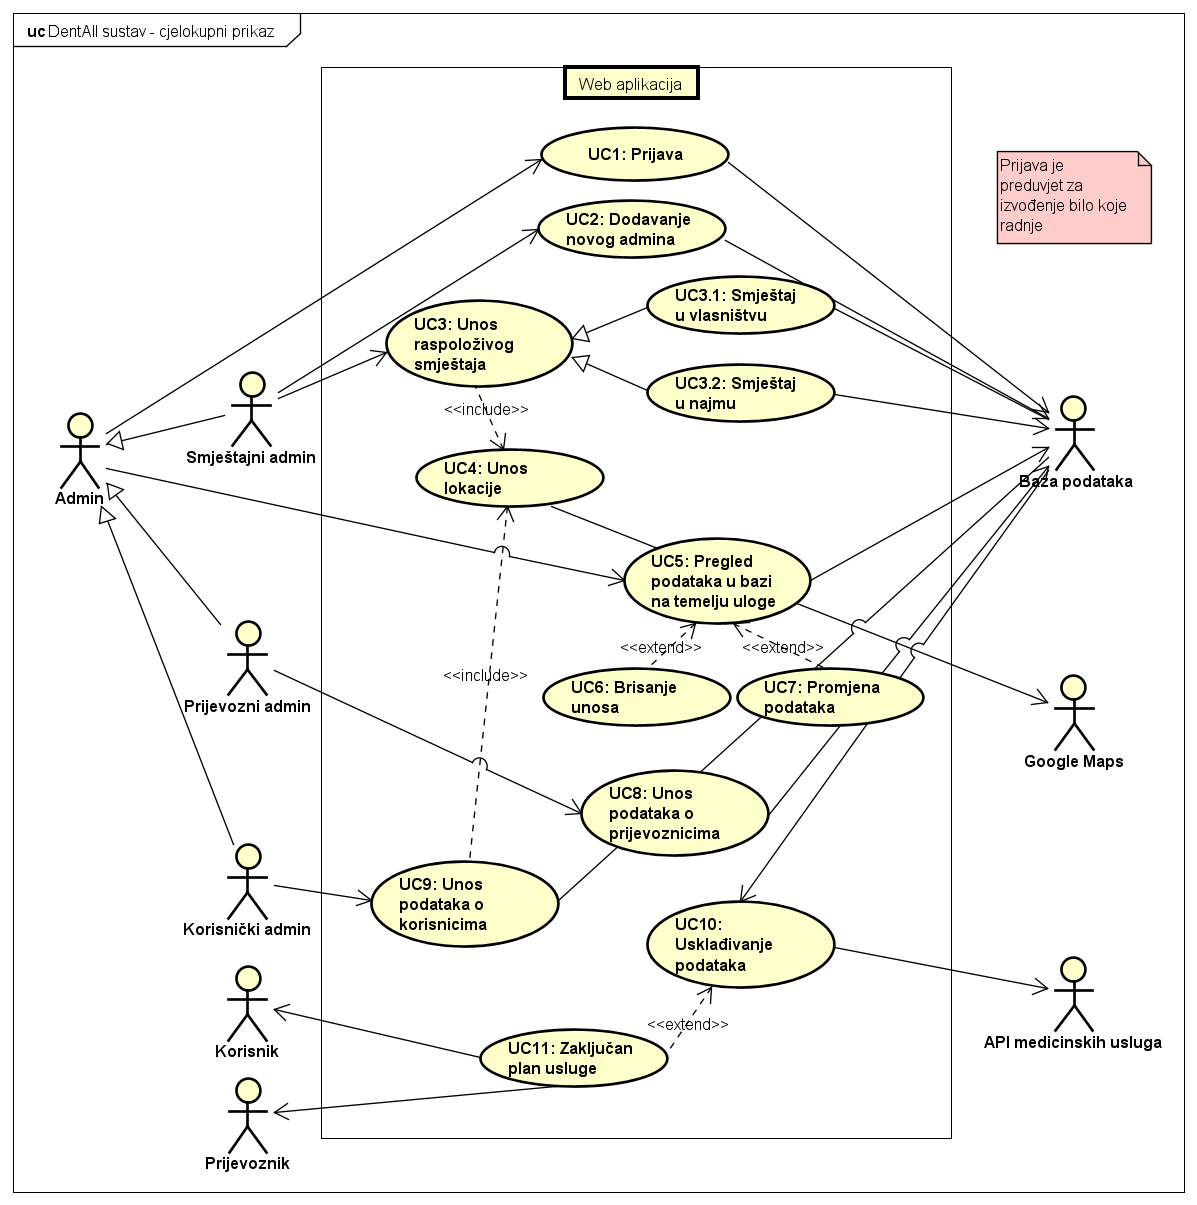
\includegraphics[width=\linewidth]{slike/Cjelokupni-prikaz-1.PNG} 
					\centering
					\caption{Sveobuhvatni prikaz}
					\label{fig:sveobuhvatniPrikaz}
				\end{figure}
				
				\begin{figure}[H]
					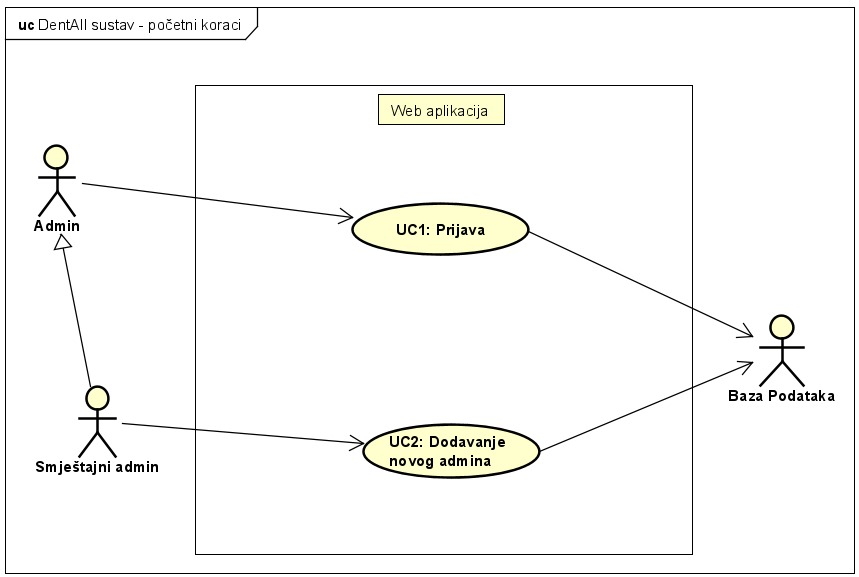
\includegraphics[width=\linewidth]{slike/DentAll_Pocetni-Koraci.PNG} 
					\centering
					\caption{Početni koraci}
					\label{fig:pocetniKoraci}
				\end{figure}
				
				\begin{figure}[H]
					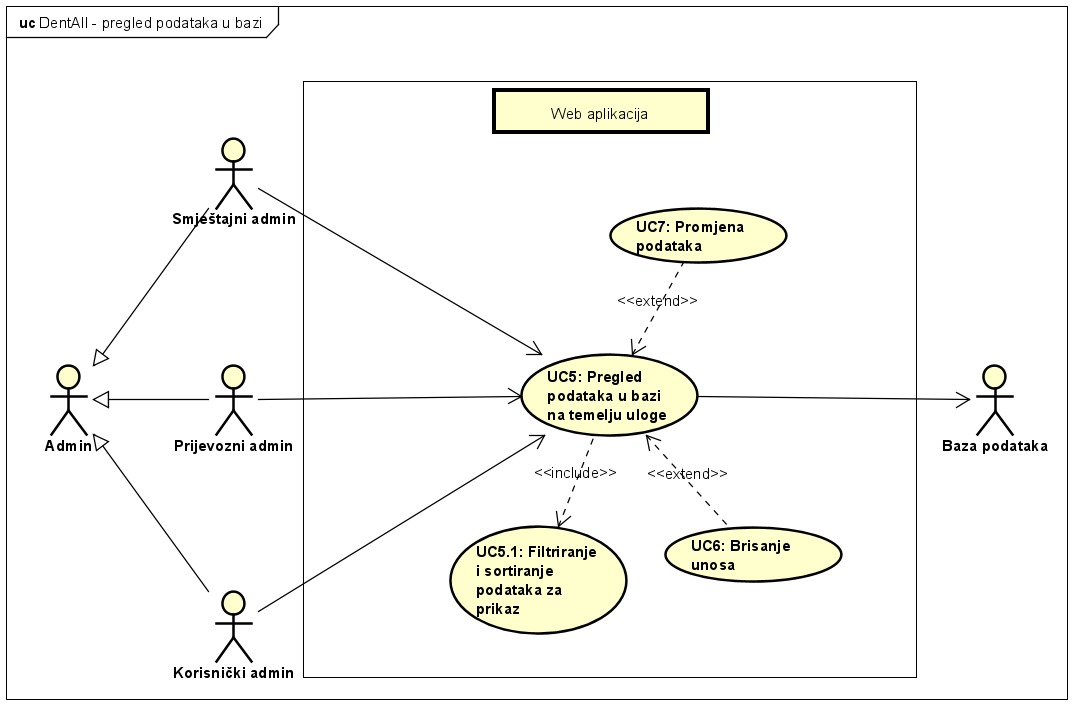
\includegraphics[width=\linewidth]{slike/DentAll_PregledPodatakaUBazi.PNG}
					\centering
					\caption{Pregled podataka u bazi podataka}
					\label{fig:pregledPodataka}
				\end{figure}
				
				\begin{figure}[H]
					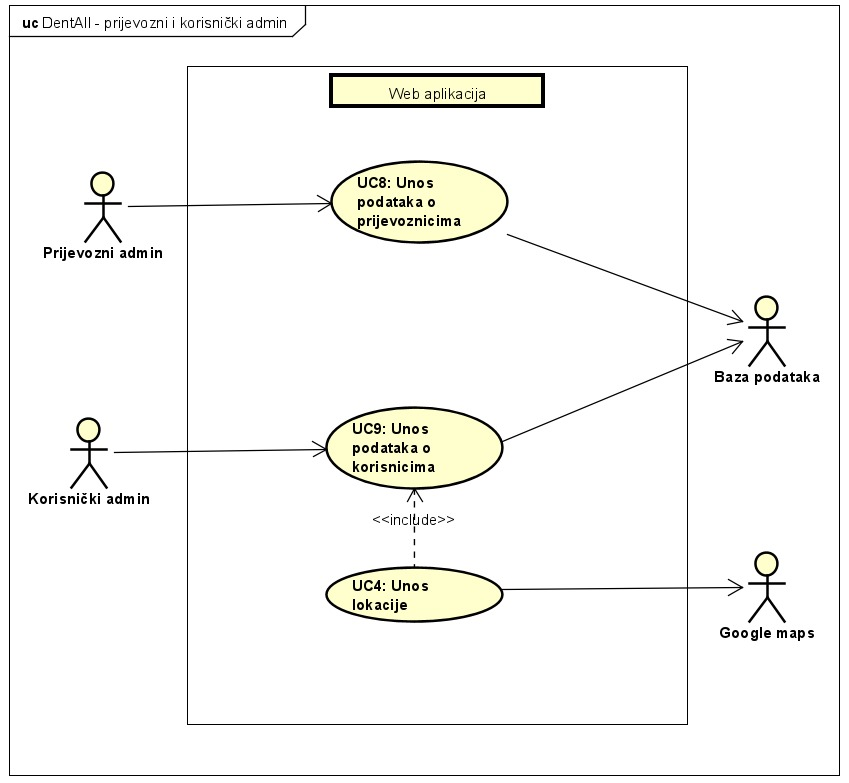
\includegraphics[width=\linewidth]{slike/DentAll_PrijevozniIKorisničkiAdmin.png}
					\centering
					\caption{Prikaz uloga korisničkog i prijevoznog administratora}
					\label{fig:prijevozniIKorisničkiAdmin}
				\end{figure}
				
				\begin{figure}[H]
					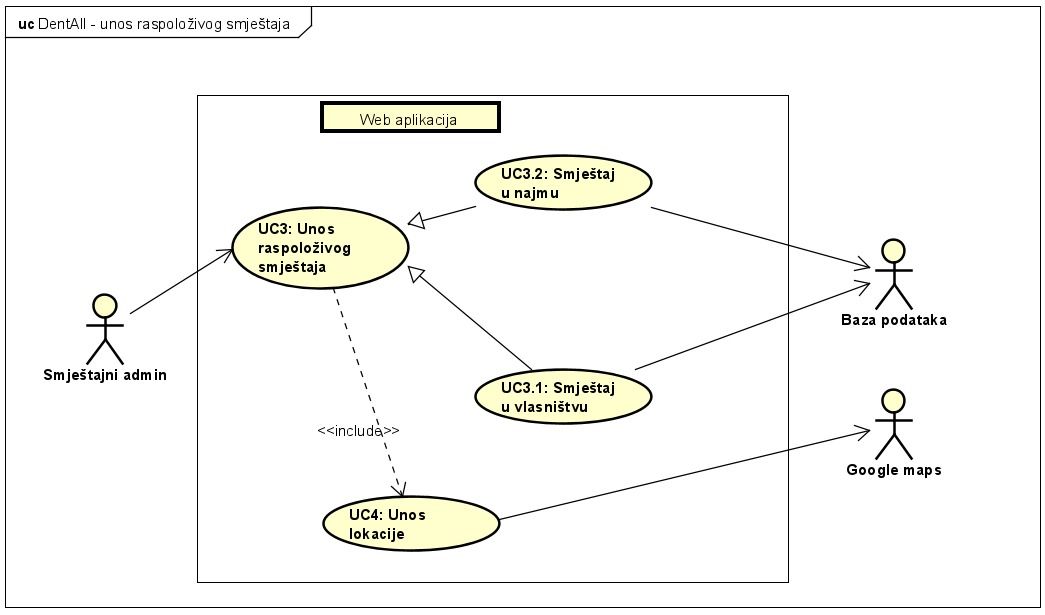
\includegraphics[width=\linewidth]{slike/DentAll_UnosRaspoloživogSmještaja.png} 
					\centering
					\caption{Prikaz unosa raspooloživog smještaja}
					\label{fig:unosSmještaja}
				\end{figure}
				
				\begin{figure}[H]
					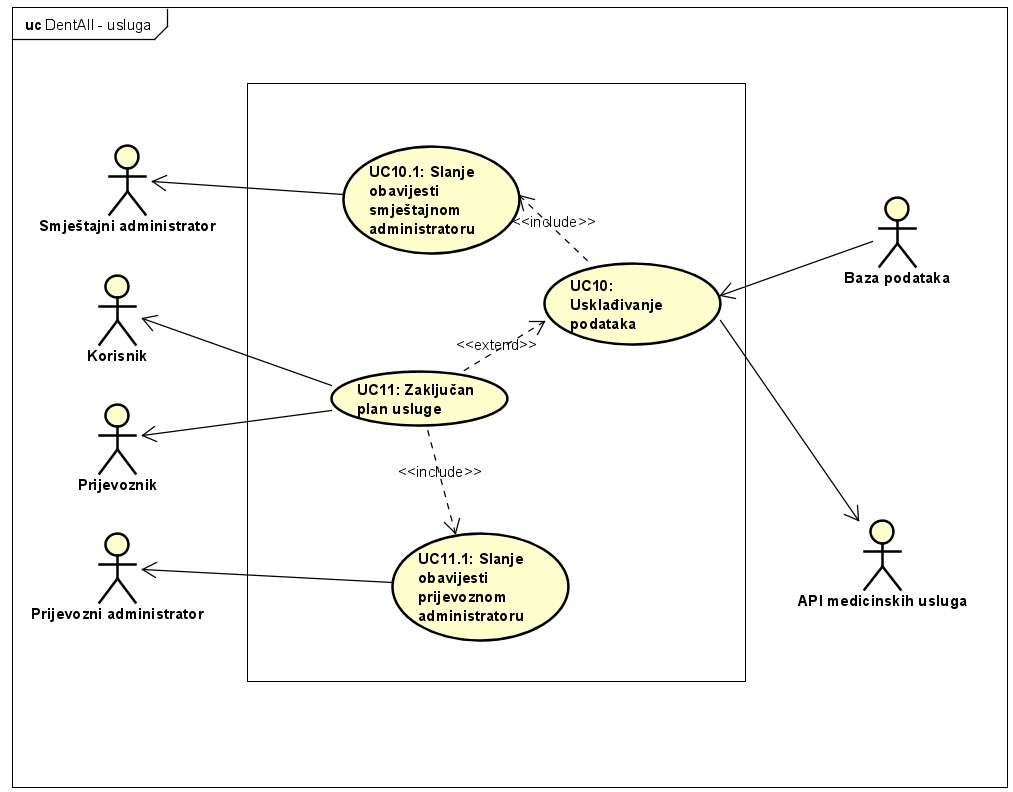
\includegraphics[width=\linewidth]{slike/DentAll_Usluga.png}
					\centering
					\caption{Prikaz korisničke strane}
					\label{fig:korisnik}
				\end{figure}
				
			\subsection{Sekvencijski dijagrami}
				
				\textbf{\textit{dio 1. revizije}}\\
				\textbf{UC1-Prijava}
				{Administrator unosi korisničko ime i lozinku.Web preglednik to upućuje bazi podataka na validaciju. Ako korisnički podaci nisu ispravni ili su nepoznati, korisnikova prijava nije uspjela te se ispisuje greška. Ako je prijava uspjela korisnik je preusmjeren na početnu stranicu.}
				
				\begin{figure}[H]
					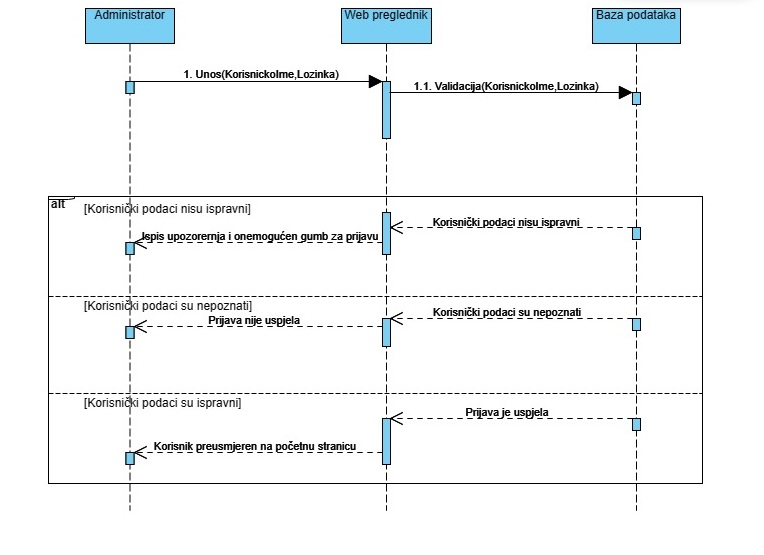
\includegraphics[width=\linewidth]{slike/DentAll_Sekvencijski-UC1-Prijava.jpeg} 
					\centering
					\caption{Sekvencijski dijagram UC1-Prijava}
					\label{fig:Sekvencijski dijagram UC1}
				\end{figure}
				
				\newpage
				
					\textbf{UC2-Dodavanje novog administratora}
					
					{Smještajni administrator prvo se mora prijaviti (UC1-Prijava). Nakon toga odabire opciju za dodavanje novog korisnika te upisuje njegove podatke. Dok nije unesen korisnik u dobrom formatu, korisniku (smještajnom administratoru) se ispisuje upozorenje o krivom formatu. Nakon što se unese dobar format, smještajni administrator unosi ulogu. Dok nije označena uloga ispisuje se upozorenje o neoznačenoj ulozi. Nakon što je uloga označena, smještajni administrator moram kliknuti na gumb pri čemu se šalje zahtjev za unos u bazu podataka. Baza  podataka može vratiti grešku te se ispisuje poruka o grešci korisniku ili se može ponovno poslati zahtjev za unos u bazu podataka. Nakon što je korisnik uspješno unesen, smještajnom administratoru se sva polja vračaju na početnu vrijednost.}
				
				\begin{figure}[H]
					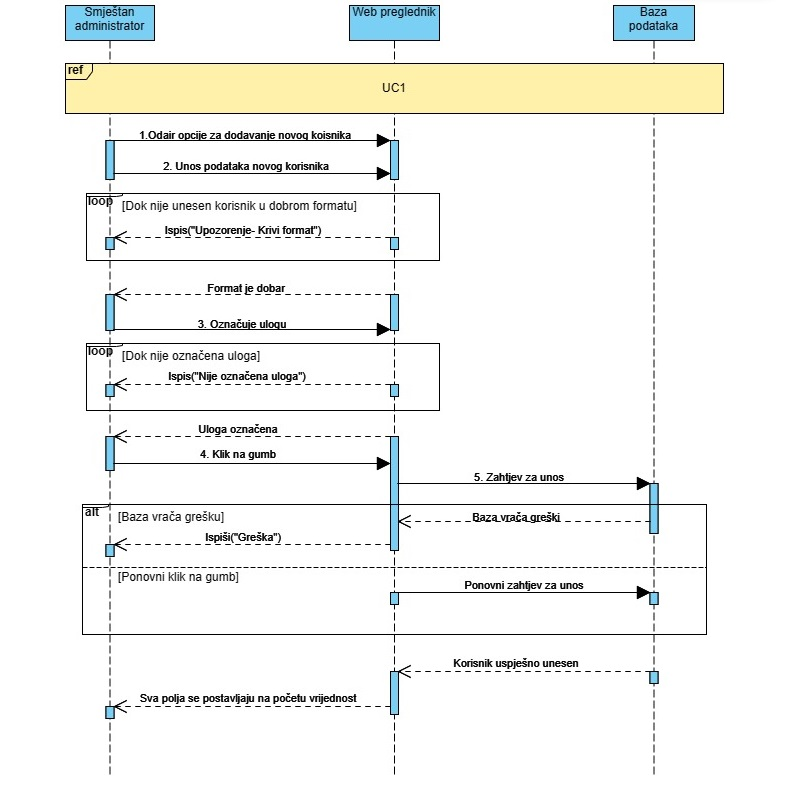
\includegraphics[width=\linewidth]{slike/DentAll-Sekvencijski-uc2-Dodavanje_novog_administratora.jpeg}
					\centering
					\caption{Sekvencijski dijagram UC2-Dodavanje novog administratora}
					\label{fig:Sekvencijski dijagram UC2}
				\end{figure}
				
				\newpage
				
				
				\textbf{UC3-Unos razpoloživog smještaja}
				
				{Smještajni administrator se prvo se mora prijaviti(UC1-Prijava). Nakon toga smještajni administrator odabire opciju dodavanja novog smještaja te odabire tip stana. Web preglednik pošalje zahtjev bazi podataka za unos te baza ako nije odabran tip šalje povratnu informaciju pregledniku, a preglednik korisniku ispiše upozorenje o odabiru tipa. Ako je uspješno odabran tip , sljedeće se unosi kategorija, te ponovno šalje zahtjev za unos, ako nije odabrana kategorija ispisuje se upozorenje o odabiru kategorije. Nakon što je kategorija uspješno odabrana, smještajni administrator odabire maksimalan kapacitet i unosi informacije o zgradi,web preglednik ponovno pošalje zahtjev za unos, te baza podataka može poslati grešku nazad u slučaju ako je krivi format unosa. Na kraju smještajni administrator odabire tip vlasništva, čime se detaljnije bave UC3.1 -Smještaj u vlasništvu i UC3.2 - Smještaj u najmu.}
				
				\begin{figure}[H]
					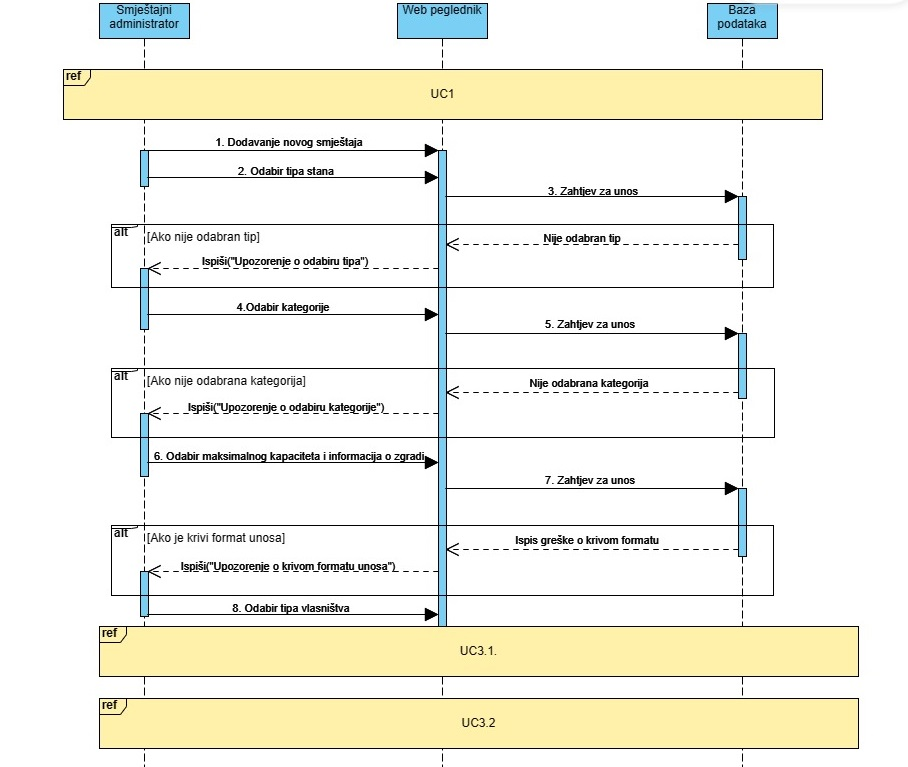
\includegraphics[width=\linewidth]{slike/DentAll-Sekvencijski-uc3-unos_raspoloživog_smještaja.jpg}
					\centering
					\caption{Sekvencijski dijagram UC3-Unos raspoloživog smještaja}
					\label{fig:Sekvencijski dijagram UC3}
				\end{figure}
				
				\eject
	
		\section{Ostali zahtjevi}
		
			\textbf{\textit{dio 1. revizije}}\\
		 
			 \textit{Nefunkcionalni zahtjevi i zahtjevi domene primjene dopunjuju funkcionalne zahtjeve. Oni opisuju \textbf{kako se sustav treba ponašati} i koja \textbf{ograničenja} treba poštivati (performanse, korisničko iskustvo, pouzdanost, standardi kvalitete, sigurnost...). Primjeri takvih zahtjeva u Vašem projektu mogu biti: podržani jezici korisničkog sučelja, vrijeme odziva, najveći mogući podržani broj korisnika, podržane web/mobilne platforme, razina zaštite (protokoli komunikacije, kriptiranje...)... Svaki takav zahtjev potrebno je navesti u jednoj ili dvije rečenice.}
			 \begin{packed_item}
                \item Aplikacija mora biti u mogućnosti grafički prikazati geografski položaj nekretnine korištenjem Google Maps/Open Maps usluge.
                \item Aplikacijsko sučelje mora imati mogućnost preuzimanja detalja korisnikovih tretmana iz aplikacije za evidenciju medicinskih usluga.
                \item Sustav treba biti jednostavan za korištenje.
                \item Korištenje sustava ne smije narušavati njegovu funkcionalnost i rad.
                \item Svi privatni podatci u sustavu moraju biti zaštićeni.
                \item Lozinke moraju biti sigurno spremljene u bazi.
                \item Nadogradnja sustava ne smije narušavati njegove postojeće funkcije.
                \item Sustav treba podržavati istovremeni rad više korisnika.
		  	\end{packed_item}
			 
			 
	